\PassOptionsToPackage{naturalnames}{hyperref}
\RequirePackage{luatex85}
\documentclass{article}
\usepackage{geometry}
%\usepackage{fullpage}
\usepackage{parskip}
\usepackage{physics}
\usepackage{amsmath}
\usepackage{amssymb}
\usepackage{xcolor}
\usepackage[colorlinks,linkcolor=blue,citecolor=green]{hyperref}
\usepackage{array}
\usepackage{longtable}
\usepackage{multirow}
\usepackage{comment}
\usepackage{graphicx}
\usepackage{cite}
\usepackage{amsfonts}
\usepackage{bm}
\usepackage{slashed}
\usepackage{dsfont}
\usepackage{mathtools}
\usepackage[compat=1.1.0]{tikz-feynman}
\usepackage{simplewick}
%\usepackage{fourier}
%\usepackage{slashbox}
%\usepackage{intent}
\usepackage{mathrsfs}
\usepackage{xparse}
\usepackage{enumerate}
%\usepackage{axodraw4j}


\geometry{left=0.9cm,right=0.9cm,top=1.5cm,bottom=2cm}

\newcommand{\gm}{\gamma^{\mu}}
\newcommand{\gn}{\gamma^{\nu}}
\newcommand{\gs}{\gamma^{\sigma}}
\newcommand{\gr}{\gamma^{\rho}}
\newcommand{\gnr}{g^{\nu\rho}}
\newcommand{\gmr}{g^{\mu\rho}}
\newcommand{\gms}{g^{\mu\sigma}}
\newcommand{\gns}{g^{\nu\sigma}}
\newcommand{\vbp}{\vb{p}}
\newcommand{\vbk}{\vb{k}}
\newcommand{\g}{\gamma}
\renewcommand{\a}{\alpha}
\renewcommand{\b}{\beta}
\renewcommand{\t}{\theta}
\newcommand{\la}{\lambda}
\newcommand{\p}{\phi}
\newcommand{\vp}{\varphi}
\newcommand{\s}{\sigma}
\newcommand{\G}{\Gamma}
\newcommand{\pars}{\slashed\partial}
\newcommand{\ps}{\slashed p}
\newcommand{\ks}{\slashed k}
\newcommand{\lag}{\mathcal{L}}
\newcommand{\da}{^{\dagger}}
\newcommand{\sm}{^{\mu}}
\newcommand{\sn}{^{\nu}}
\newcommand{\smn}{^{\mu\nu}}
\newcommand{\Dm}{D^{\mu}}
\newcommand{\dm}{\partial^{\mu}}
\newcommand{\Asquare}{A^{\mu}A_{\mu}}
\newcommand{\partialsquare}[2]{\partial^{\mu}{#1}\partial_{\mu}{#2}}

\title{Hydrogen}
\author{Yingsheng Huang}
\begin{document}
\maketitle
QED Lagrangian is 
\begin{align}
  \lag_{QED}=\bar l(i\slashed D-m)l+\bar N(i D^0)N-\lag_{\gamma}
  \label{}
\end{align}
Set the NRQED Lagrangian as (take large $M$ limit where $M$ is the mass of the proton/hydrogen nucleus)
\begin{align}
  \lag_{NRQED}=\psi^{\dagger}(iD_0+\frac{\vb{D}^2}{2m})\psi+\bar N(iD_0)N+\lag_{4-fer}+\lag_{\gamma}
  \label{}
\end{align}
The box %and crossed box 
diagram for NRQED process is
\begin{align*}
  i\mathcal{M}_{NRQED}&=\feynmandiagram[horizontal=i1 to f1,layered layout,inline=($(a)!0.5!(c)$),medium]{
	i1[particle=$P_N$] -- [double distance=1pt] a -- [double distance=1pt,momentum=$P_N-k$] b -- [double distance=1pt] f1[particle=$P_N$],
	i2[particle=$p_1$] -- [fermion] c -- [fermion,momentum'=$p1+k$] d -- [fermion] f2[particle=$p_2$],
	{ [same layer] a -- [photon,momentum'=$k$] c},
	{ [same layer] b-- [photon,rmomentum=$k-q$] d},
  };\\
  &=e^4\bar u_N(P_N)\frac{1+\g^0}{2}u_N(P_N)\psi^{\dagger}(p_2)\int[\dd k]\frac{1}{\vb{k}^2(\vb{k}-\vb{q})^2(-k^0+i\epsilon)(p_1^0+k^0-m-\frac{\vb{p_1+k}^2}{2m}+i\epsilon)}\psi(p_1)\\
  &=-ie^4\bar u_N(P_N)\frac{1+\g^0}{2}u_N(P_N)\psi^{\dagger}(p_2)\int\frac{\dd^3k}{(2\pi)^3}\frac{1}{\vb{k}^2(\vb{k}-\vb{q})^2(E_1-\frac{\vb{p_1+k}^2}{2m})}\psi(p_1)\\
  &=-ie^4\bar u_N(P_N)\frac{1+\g^0}{2}u_N(P_N)\psi^{\dagger}(p_2)\int\frac{\dd^3k}{(2\pi)^3}\frac{1}{(\vb{k}-\vb{p_1})^2(\vb{k}-\vb{p_2})^2(E_1-\frac{\vb{k}^2}{2m})}\psi(p_1)
\end{align*}
\clearpage 
The box and crossed box diagram for QED process is
\begin{align*}
  i\mathcal{M}_1&=\feynmandiagram[horizontal=i1 to f1,layered layout,inline=($(a)!0.5!(c)$),medium]{
	i1[particle=$P_N$] -- [double distance=1pt] a -- [double distance=1pt,momentum=$P_N-k$] b -- [double distance=1pt] f1[particle=$P_N$],
	i2[particle=$p_1$] -- [fermion] c -- [fermion,momentum'=$p1+k$] d -- [fermion] f2[particle=$p_2$],
	{ [same layer] a -- [photon,momentum'=$k$] c},
	{ [same layer] b-- [photon,rmomentum=$k-q$] d},
  };\\
  &=e^4\bar u_N(P_N)\frac{1+\g^0}{2}u_N(P_N)u_e^{\dagger}(p_2)\int[\dd k]\frac{(\slashed p_1+\slashed k+m)\g^0}{\vb{k}^2(\vb{k}-\vb{q})^2[(p_1+k)^2-m^2+i\epsilon](-k^0+i\epsilon)}u_e(p_1)\\
  &=e^4\bar u_N(P_N)\frac{1+\g^0}{2}u_N(P_N)u_e^{\dagger}(p_2)\int[\dd k]\frac{2p_1^0+\slashed k\g^0}{\vb{k}^2(\vb{k}-\vb{q})^2[(p_1+k)^2-m^2+i\epsilon](-k^0+i\epsilon)}u_e(p_1)\\
  &=ie^4\bar u_N(P_N)\frac{1+\g^0}{2}u_N(P_N)u_e^{\dagger}(p_2)\int\frac{\dd^3 k}{(2\pi)^3}\frac{p_1^0+k_i\g^i\g^0+\sqrt{(\vb{k}+\vb{p_1})^2+m^2}}{2\vb{k}^2(\vb{k}-\vb{q})^2[(\vb{k}+\vb{p_1})^2+m^2-p_1^0\sqrt{(\vb{k}+\vb{p_1})^2+m^2}]}u_e(p_1)\\
  &=ie^4\bar u_N(P_N)\frac{1+\g^0}{2}u_N(P_N)u_e^{\dagger}(p_2)\int\frac{\dd^3 k}{(2\pi)^3}\frac{p_1^0+(k_i-p_{1i})\g^i\g^0+\sqrt{\vb{k}^2+m^2}}{2(\vb{k}-\vb{p_1})^2(\vb{k}-\vb{p_2})^2[\vb{k}^2+m^2-p_1^0\sqrt{\vb{k}^2+m^2}]}u_e(p_1)
 \end{align*}
 $i\mathcal{M}_1$ has infrared log divergence and no ultraviolet divergence.
 \begin{align*}
  i\mathcal{M}_2&=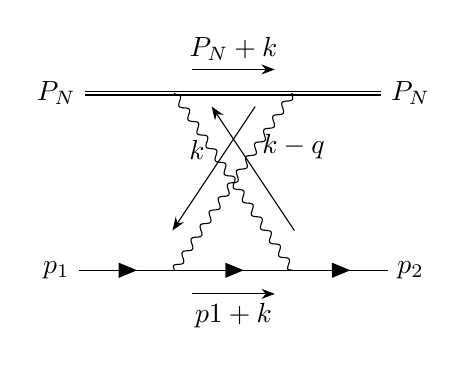
\begin{tikzpicture}[baseline=($(a)!0.5!(c)$)]
	\begin{feynman}
	  \diagram[horizontal=i1 to f1,layered layout,medium]{
		i1[particle=$P_N$] -- [double distance=1pt] a -- [double distance=1pt,momentum=$P_N+k$] b -- [double distance=1pt] f1[particle=$P_N$],
	i2[particle=$p_1$] -- [fermion] c -- [fermion,momentum'=$p1+k$] d -- [fermion] f2[particle=$p_2$],
	{ [same layer] a --[draw=none] c},
	{ [same layer] b-- [draw=none] d},
  };
	  \diagram*{
		(a) -- [photon,rmomentum=$k-q$] (d),
		(b) -- [photon,momentum'=$k$] (c),
	  };
	\end{feynman}
  \end{tikzpicture}\\
  &=e^4\bar u_N(P_N)\frac{1+\g^0}{2}u_N(P_N)u_e^{\dagger}(p_2)\int[\dd k]\frac{(\slashed p_1+\slashed k+m)\g^0}{\vb{k}^2(\vb{k}-\vb{q})^2[(p_1+k)^2-m^2+i\epsilon](k^0+i\epsilon)}u_e(p_1)\\
  &=e^4\bar u_N(P_N)\frac{1+\g^0}{2}u_N(P_N)u_e^{\dagger}(p_2)\int[\dd k]\frac{2p_1^0+\slashed k\g^0}{\vb{k}^2(\vb{k}-\vb{q})^2[(p_1+k)^2-m^2+i\epsilon](k^0+i\epsilon)}u_e(p_1)\\
  &=-ie^4\bar u_N(P_N)\frac{1+\g^0}{2}u_N(P_N)u_e^{\dagger}(p_2)\int\frac{\dd^3 k}{(2\pi)^3}\frac{p_1^0+k_i\g^i\g^0-\sqrt{(\vb{k}+\vb{p_1})^2+m^2}}{2\vb{k}^2(\vb{k}-\vb{q})^2[(\vb{k}+\vb{p_1})^2+m^2+p_1^0\sqrt{(\vb{k}+\vb{p_1})^2+m^2}]}u_e(p_1)\\
  &=-ie^4\bar u_N(P_N)\frac{1+\g^0}{2}u_N(P_N)u_e^{\dagger}(p_2)\int\frac{\dd^3 k}{(2\pi)^3}\frac{p_1^0+(k_i-p_{1i})\g^i\g^0-\sqrt{\vb{k}^2+m^2}}{2(\vb{k}-\vb{p_1})^2(\vb{k}-\vb{p_2})^2[\vb{k}^2+m^2+p_1^0\sqrt{\vb{k}^2+m^2}]}u_e(p_1)
 \end{align*}
 $i\mathcal{M}_2$ has no infrared or ultraviolet divergence.
%\includegraphics[width=0.5\textwidth]{NRQED.eps}
 \begin{align*}
 i\mathcal{M}_1+i\mathcal{M}_2&=ie^4\bar u_N(P_N)\frac{1+\g^0}{2}u_N(P_N)u_e^{\dagger}(p_2)\int\frac{\dd^3 k}{(2\pi)^3}\frac{{p_1^0}^2+k^2+m^2+(k_i-p_{1i})p_1^0\g^i\g^0}{(\vb{k}-\vb{p_1})^2(\vb{k}-\vb{p_2})^2[\vb{k}^2+m^2-{p_1^0}^2]\sqrt{\vb{k}^2+m^2}}u_e(p_1)\\
 &=ie^4\bar u_N(P_N)\frac{1+\g^0}{2}u_N(P_N)u_e^{\dagger}(p_2)\int\frac{\dd^3 k}{(2\pi)^3}\frac{{p_1^0}^2+k^2+m^2+(k_i-p_{1i})p_1^0\g^i\g^0}{(\vb{k}-\vb{p_1})^2(\vb{k}-\vb{p_2})^2[\vb{k}^2-\vb{p_1}^2]\sqrt{\vb{k}^2+m^2}}u_e(p_1)
 \end{align*}

\end{document}


